\documentclass[10.5pt,a4paper]{article}
\usepackage[a4paper,margin=2cm]{geometry}
\usepackage[T1]{fontenc}
\usepackage[utf8]{inputenc}
\usepackage{lmodern}
\usepackage{amsmath,amssymb,bm}
\usepackage{graphicx}
\usepackage{booktabs}
\usepackage{caption}
\usepackage{subcaption}
\usepackage[hidelinks]{hyperref}
\usepackage{enumitem}
\usepackage{xcolor}
\setlist{nosep,leftmargin=1.2em}
\captionsetup{font=small,labelfont=bf}
\setlength{\parskip}{0.35em}
\setlength{\parindent}{0pt}
\graphicspath{{../figures/}}

% ---------------------------------------------------------------- fill in --
\newcommand{\authors}{Paula Blasco}
\newcommand{\githuburl}{\url{https://github.com/PaulaBlasco888/ds-obstacle-avoidance-3d}}
\newcommand{\videourl}{\textcolor{red}{[YouTube link]}}

\begin{document}

% ================================================================== COVER ==
\begin{titlepage}
\centering
\vspace*{3cm}
{\large Universidad Carlos III de Madrid\par}
{\large Robot's Control Architectures, Laboratory Project\par}
\vspace{2.5cm}
{\LARGE\bfseries 3D Obstacle Avoidance and Control\\[0.3em] using Dynamical Systems\par}
\vspace{2cm}
{\large \authors\par}
\vspace{0.5cm}
{\large November 2026\par}
\vfill
\begin{tabular}{rl}
Source code: & \githuburl \\
Video: & \videourl
\end{tabular}
\vspace{2cm}
\end{titlepage}

% ============================================================ 1. INTRO ======
\section{Introduction and problem statement}

The goal of this project is to move a robot's end-effector from any starting point to a target
$x^*\in\mathbb{R}^3$ while avoiding an obstacle, without planning a path beforehand. Instead of a
trajectory, the robot follows a \emph{dynamical system} (DS) $\dot x = f(x)$ that gives the desired
velocity at every point. If $f$ is globally asymptotically stable at $x^*$, the robot reaches the
target from anywhere and recovers naturally from perturbations. Obstacles are handled by locally
\emph{modulating} that velocity field, $\dot x = M(x)f(x)$, which is cheap enough to be evaluated
at every control step.

We put together the two lab sessions. In Lab~1 we learned stable non-linear DS from demonstrations
(SEDS and LPV-DS). The obstacle-avoidance code from Lab~2 only modulated a linear attractor
$f(x)=-(x-x^*)$, which goes straight to the target. Our work had four steps:
\begin{enumerate}
\item Port the LPV-DS learning to Python and plug it into the 2D obstacle-avoidance package, replacing
the linear attractor.
\item Learn a 3D LPV-DS from real robot demonstrations and check its stability, both analytically
and empirically.
\item Implement the 3D obstacle model ($\Gamma(x)$, $n(x)$, orthonormal basis, $D(x)$,
$M(x)\in\mathbb{R}^{3\times 3}$) ourselves and simulate the end-effector as a point.
\item Use the modulated DS to drive a Franka Emika Panda through its Jacobian,
$\dot q = J^{+}(q)\dot x_{mod}$, respecting the real joint limits.
\end{enumerate}

% ======================================================= 2. FORMULATION =====
\section{Mathematical formulation in $\mathbb{R}^3$}

\paragraph{Nominal DS (LPV-DS).} Following Figueroa and Billard~\cite{figueroa}, the DS is a
state-dependent mixture of linear systems:
\begin{equation}
f(x)=\sum_{k=1}^{K}\gamma_k(x)\,(A_k x+b_k),\qquad
\gamma_k(x)=\frac{\pi_k\,\mathcal{N}(x\,|\,\mu_k,\Sigma_k)}{\sum_j \pi_j\,\mathcal{N}(x\,|\,\mu_j,\Sigma_j)} .
\end{equation}
The weights $\gamma_k$ come from a Gaussian mixture model (GMM) fitted to the demonstrated
positions, so $\gamma_k\ge 0$ and $\sum_k\gamma_k=1$. The matrices $A_k$ are found by minimising
$\sum_n\|f(x_n)-\dot x_n\|$ over the demonstrations, subject to
\begin{equation}
A_k^{T}P+PA_k\preceq-\varepsilon I,\qquad b_k=-A_k x^*,\qquad k=1,\dots,K,
\label{eq:constr}
\end{equation}
with $P\succ 0$ fixed beforehand. For a fixed $P$ these are linear matrix inequalities, so the problem
is a convex semidefinite program.

\paragraph{Stability.} Take $V(x)=(x-x^*)^{T}P(x-x^*)$, which is positive definite. With
$b_k=-A_kx^*$ we get $f(x)=\sum_k\gamma_k(x)A_k(x-x^*)$, so $f(x^*)=0$ and
\begin{equation}
\dot V(x)=\sum_{k=1}^{K}\gamma_k(x)\,(x-x^*)^{T}\big(A_k^{T}P+PA_k\big)(x-x^*)
\;\le\; -\varepsilon\,\|x-x^*\|^2<0\quad \forall x\neq x^* ,
\end{equation}
because every term is negative and the $\gamma_k$ are a convex combination. $V$ is therefore a global
Lyapunov function and $x^*$ is globally asymptotically stable. With $P=I$ (the QLF of the original
paper) the robot would be forced to always get closer to $x^*$ in Euclidean distance, which several
demonstrated shapes do not do. So we first learn $P$ with a second convex problem that makes the
demonstrations agree with $\dot V<0$ as much as possible:
$\min_P \sum_n \max\!\big(0,\ \hat{x}_n^{T}P\,\hat{\dot x}_n+0.05\big)$ s.t.
$P\succeq 0.2\,I,\ \mathrm{tr}(P)=3$, where $\hat{\cdot}$ denotes unit vectors.

\paragraph{Obstacle.} The obstacle is an ellipsoid with centre $c$, orientation $R$, semi-axes $a_i$ and
a safety factor $s_f$. In its local frame $\tilde x = R^{T}(x-c)$:
\begin{equation}
\Gamma(x)=\sum_{i=1}^{3}\left(\frac{\tilde x_i}{s_f\,a_i}\right)^{2},\qquad
n(x)=\frac{\nabla\Gamma(x)}{\|\nabla\Gamma(x)\|},\qquad
\nabla\Gamma = R\left[\frac{2\tilde x_i}{(s_f a_i)^2}\right]_{i}.
\end{equation}
$\Gamma=1$ on the (enlarged) surface, $\Gamma>1$ outside and $\Gamma<1$ inside. The normal is completed
to a right-handed orthonormal basis $[n,e_1,e_2]$ with $e_1 = n\times h/\|n\times h\|$ and
$e_2=n\times e_1$, where $h$ is the canonical axis least aligned with $n$ (this avoids
$n\times h\approx 0$).

\paragraph{Modulation.} Following~\cite{khansari2012,huber2019}:
\begin{equation}
M(x)=E(x)D(x)E(x)^{-1},\quad E=[\,r\;\;e_1\;\;e_2\,],\quad
D=\mathrm{diag}\Big(1-\tfrac{1}{\Gamma},\;1+\tfrac{1}{\Gamma},\;1+\tfrac{1}{\Gamma}\Big),\quad
\dot x_{mod}=M(x)f(x),
\end{equation}
where $r=(x-x_{ref})/\|x-x_{ref}\|$ points away from a reference point inside the obstacle (its
centre here; for a sphere $r=n$). On the surface the first eigenvalue is zero, so the component of $f$
that would push into the obstacle disappears and only tangential motion is left. Far away
$D\to I$ and the learned DS is unchanged. Once the robot is moving away from the obstacle
($n^{T}f>0$) we set $\lambda_r=1$, so it is not slowed down after passing it.

\paragraph{Robot.} The end-effector of the Panda tracks $\dot x_{mod}$ while keeping the gripper
vertical. With $J(q)\in\mathbb{R}^{6\times 7}$ the geometric Jacobian:
\begin{equation}
\dot q = J^{\dagger}\begin{bmatrix}\dot x_{mod}\\ \omega\end{bmatrix}
+\big(I-J^{\dagger}J\big)\dot q_0,\qquad
J^{\dagger}=J^{T}\big(JJ^{T}+\lambda^2 I\big)^{-1},\qquad
\dot q_{0,i}=-k\,\frac{q_i-\bar q_i}{(\Delta q_i/2)^2},
\end{equation}
where $\omega$ is proportional to the orientation error and $\dot q_0$ keeps the redundant joint
away from its limits.

% ===================================================== 3. IMPLEMENTATION ===
\section{Implementation details and algorithm}

Everything is written in Python (NumPy, SciPy, cvxpy with the Clarabel solver, Matplotlib and the
Robotics Toolbox for Python~\cite{rtb}). The main modules are:
\begin{itemize}
\item \texttt{ds\_learning/lpvds.py}: dataset loading (same preprocessing as \texttt{ds-opt}), GMM
with EM and BIC model selection, learning of $P$, the SDP for $A_k$, and evaluation and RK4 simulation.
\item \texttt{ds\_learning/obstacle3d.py}: the ellipsoid class with $\Gamma$, $n$, the basis,
$D$, $M$ and the modulated velocity.
\item Scripts: \texttt{main\_3d.py} (3D results), \texttt{robot\_sim.py} (Panda), \texttt{test\_modulation.py}
(unit checks),\\ \texttt{session2\_lpvds\_obstacle\_2d.py} (2D) and \texttt{make\_video.py} (video).
\end{itemize}

\textbf{Practical issues.} The MATLAB code from Lab~1 needs the Statistics Toolbox, which we did not
have, so we ported it. We also wrote our own EM, because the Windows machine we used blocked some
compiled packages such as scikit-learn. In 2D we fixed the obstacle package so that its animation and
streamlines actually use the \texttt{dynamicalSystem} argument; before, it always used the linear
attractor. In 3D, a GMM fitted on positions alone mixed parts of the demonstrations that pass close
to each other in opposite directions. Following the idea of the physically-consistent GMM of
Lab~1, we cluster on $[x;\ w\,\sigma\,\dot x/\|\dot x\|]$ ($w=4$, $\sigma$ the position spread) and
keep only the position part of each Gaussian for $\gamma_k$. This halved the reproduction error.

\textbf{Control loop} (one step, $\Delta t=10$\,ms):
\begin{enumerate}
\item Read $q$ and compute $p=FK(q)$ and $x=p-t_{task}$. The demonstrations were recorded with a
different robot, so we shift the task by a constant $t_{task}$ into the Panda workspace. Since
$\dot x=f(x)$ does not depend on the origin, the learned behaviour is unchanged.
\item Evaluate $f(x)$ (LPV-DS), $\Gamma(x)$, $n$, $E$, $D$ and $\dot x_{mod}=M(x)f(x)$.
\item Compute $\dot q$ with the damped pseudo-inverse ($\lambda=0.02$) and the null-space term.
\item Scale $\dot q$ down if any joint exceeds the Panda velocity limit, integrate, and clip to the
joint limits.
\end{enumerate}

% ========================================================== 4. RESULTS =====
\section{Results and trajectory analysis}

\paragraph{2D integration (Lab Session 2).} Fig.~\ref{fig:2d} shows the same obstacle modulating
the original linear attractor and an LPV-DS learned from the S-shape dataset ($K=8$). The modulated
LPV-DS keeps the demonstrated S and goes around the obstacle. Starting from the 3 demonstrations and
3 perturbed points, all six trajectories reached the target (final error $<0.02$) with
$\Gamma_{min}\in[1.06,\,8.6]$. In our first attempt we used $P=I$, and the learned field cut through the
S. Learning $P$ fixed it.

\begin{figure}[h]
\centering
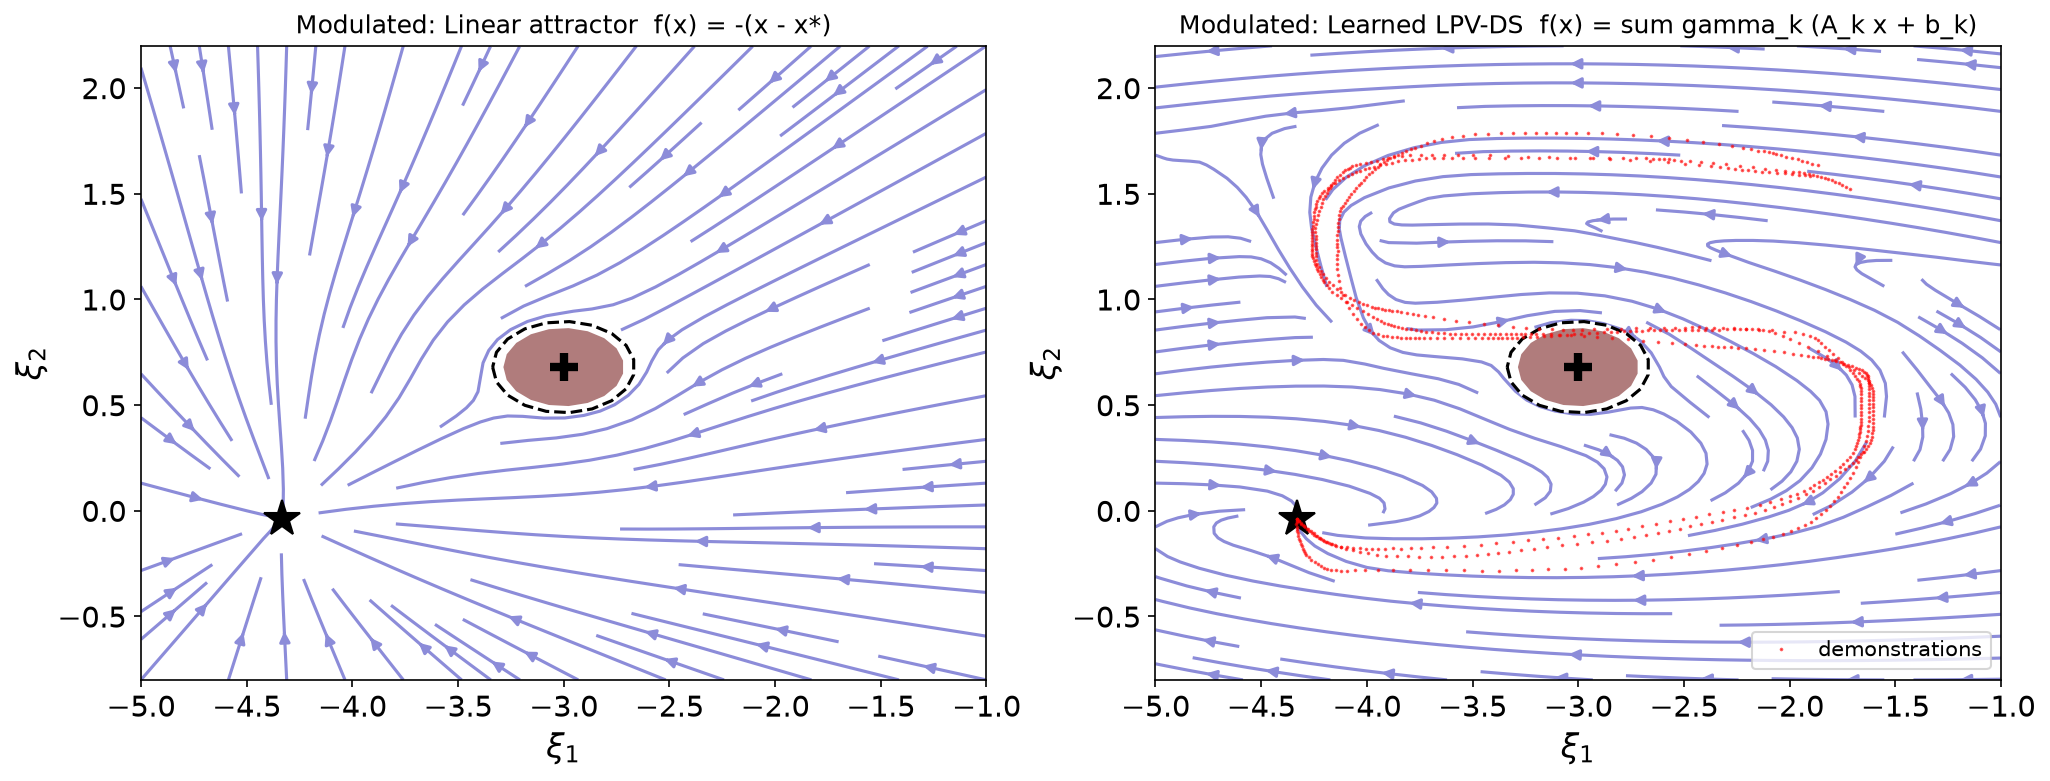
\includegraphics[width=0.74\textwidth]{sshape2d_linear_vs_lpvds.png}
\caption{2D, Lab~2 package. Left: modulated linear attractor. Right: modulated LPV-DS learned from
the red demonstrations. $\star$ is the target and $+$ the reference point of the obstacle.}
\label{fig:2d}
\end{figure}

\paragraph{3D DS.} We used \texttt{3D\_viapoint\_3} from the Lab~1 datasets (6 demonstrations,
2042 samples, a motion through a via point). We first tried the C-shape, but it moves far away from
the target before coming back, and a quadratic $V$ cannot represent that well (3 to 7\,cm of error).
The final model has $K=8$, $\varepsilon=0.01$ and $\mathrm{eig}(P)=\{0.20,\,0.29,\,2.51\}$. It
reproduces the demonstrations with a mean distance of 17\,mm (22\,mm in the worst one) along paths of
about 1.1\,m. All eight $A_k^TP+PA_k$ are negative definite (largest eigenvalue $-0.01$). As an
empirical check, $\dot V<0$ held on all of 20\,000 random points of a box around the workspace, and
$V(x(t))$ decreases monotonically along every simulated trajectory (Fig.~\ref{fig:lyap}).

\paragraph{3D avoidance.} The ellipsoid (semi-axes 6, 4.5 and 5\,cm, rotated 30$^\circ$, $s_f=1.15$)
is placed on the nominal path, so without modulation the robot would cross it (dashed lines in
Fig.~\ref{fig:3d}). We start 5 trajectories at the centre, above, below, left and right of a
demonstrated start point ($\pm3.5$\,cm). \texttt{test\_modulation.py} checks numerically that the basis
is orthonormal ($10^{-16}$), that $n$ matches the finite-difference gradient ($10^{-11}$), that
$|n^{T}Mf|/\|f\|<10^{-8}$ on the surface (no penetration) and that $M\to I$ far away.

\begin{figure}[h]
\centering
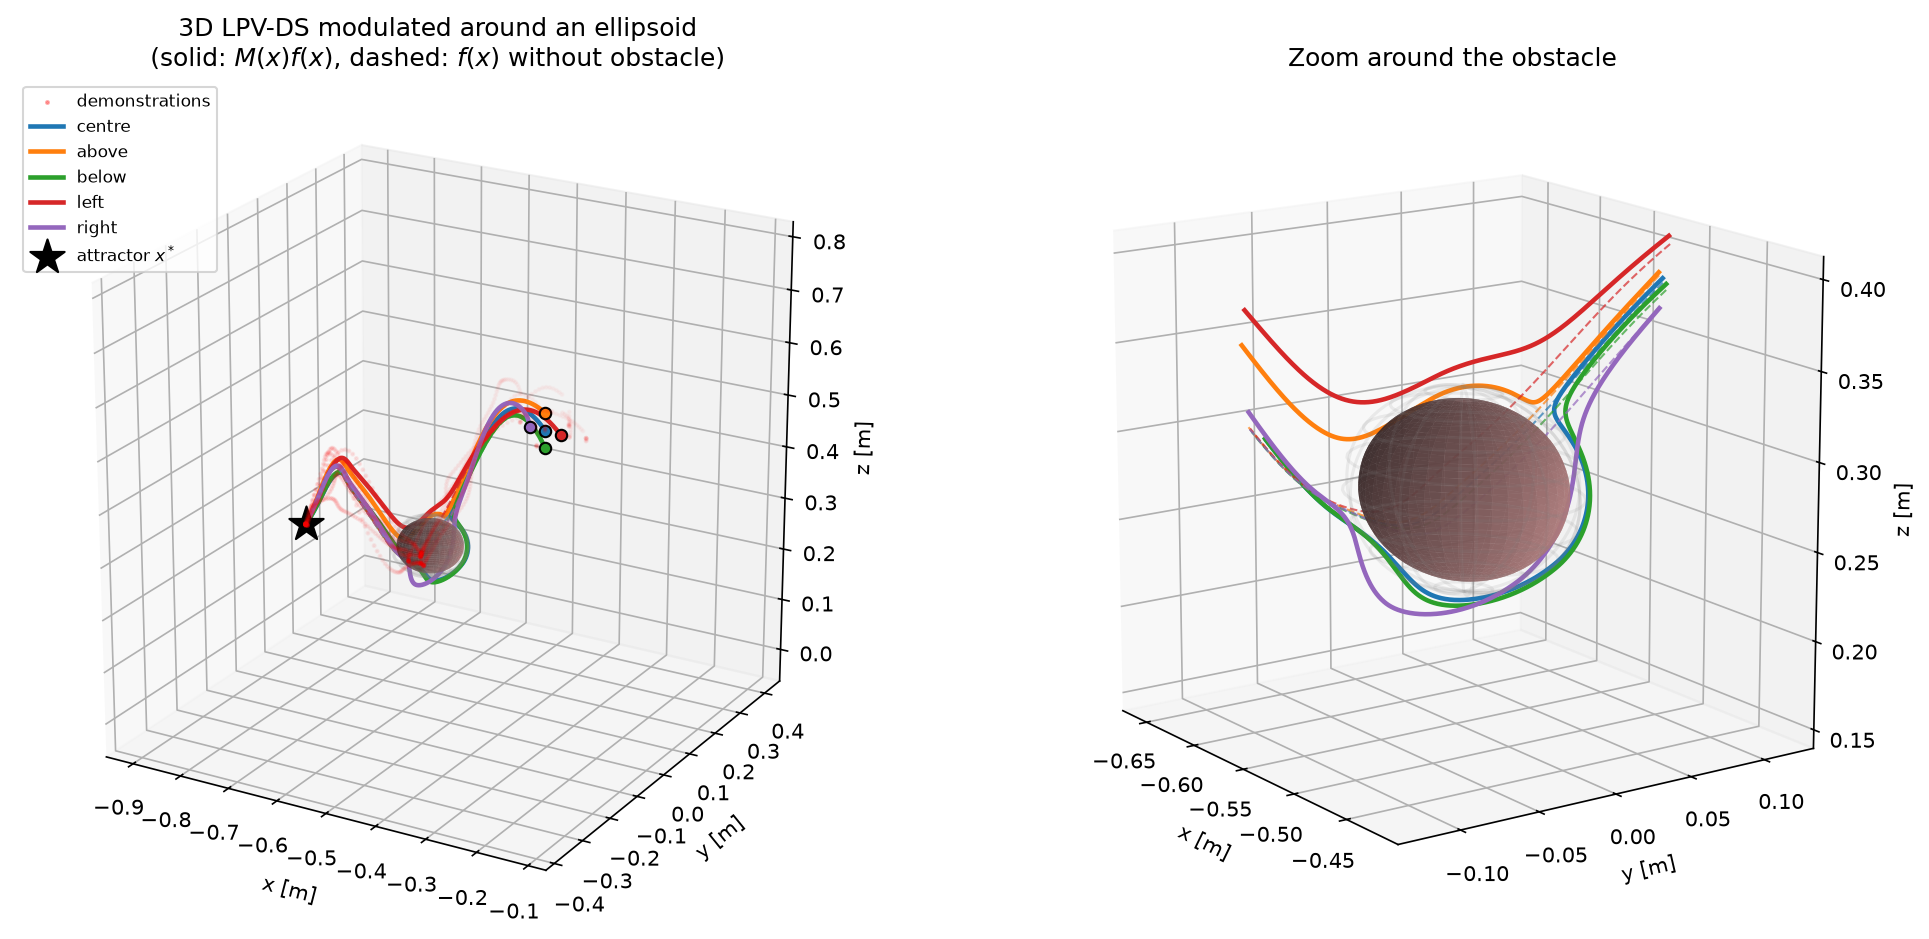
\includegraphics[width=0.92\textwidth]{viapoint3d_3d_trajectories.png}
\caption{3D LPV-DS with the ellipsoidal obstacle. Solid: $\dot x = M(x)f(x)$. Dashed: $f(x)$ without
modulation. Red dots: demonstrations. Right: zoom, where the runs go above, below and around the
sides of the obstacle.}
\label{fig:3d}
\end{figure}

\begin{figure}[!htbp]
\centering
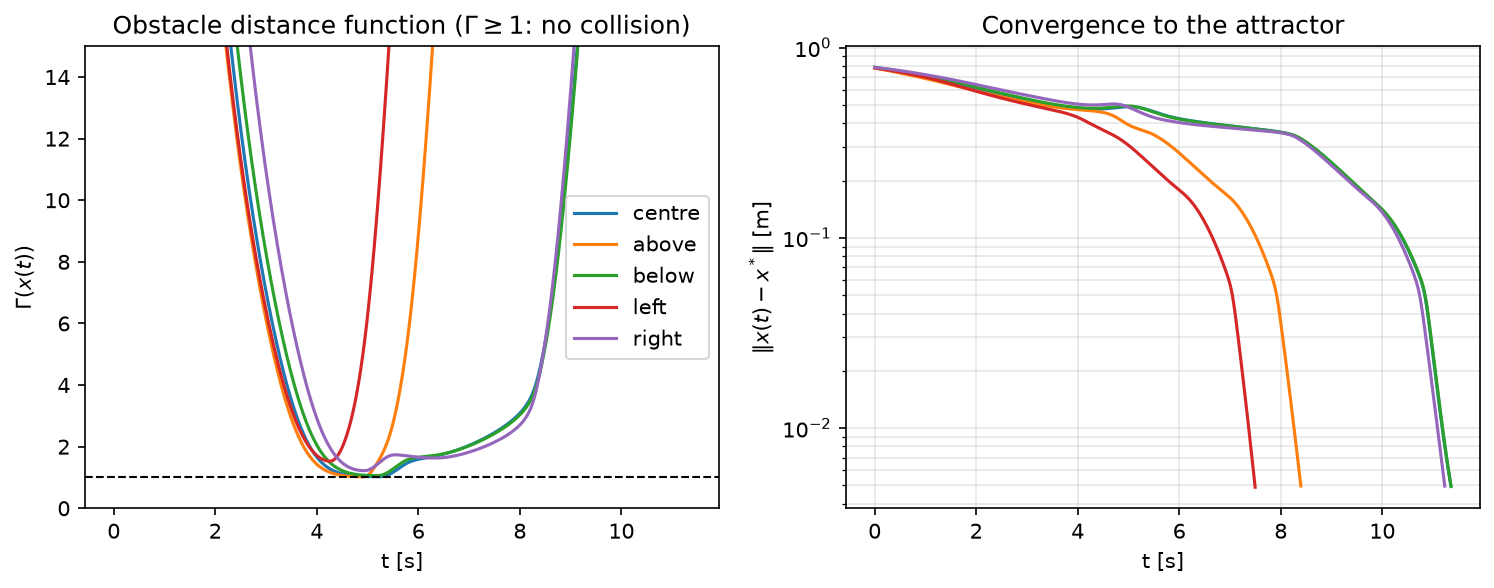
\includegraphics[width=0.6\textwidth]{viapoint3d_gamma_convergence.png}\\[0.2em]
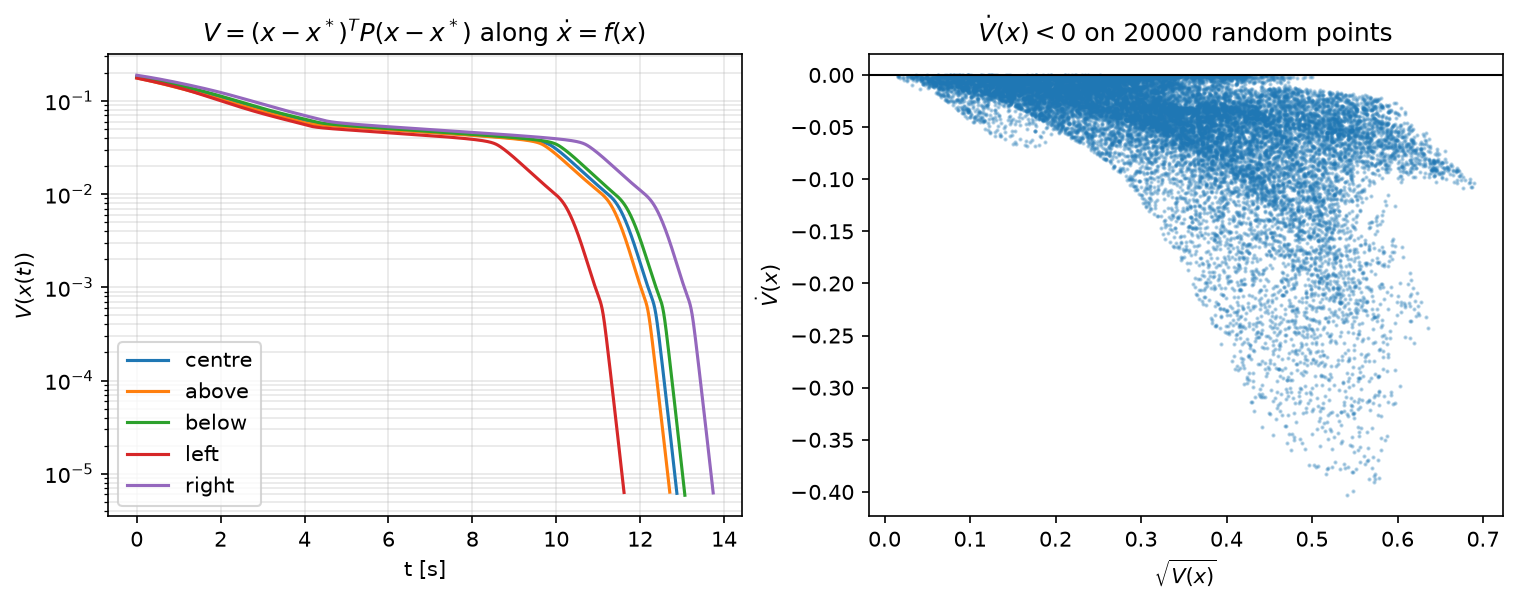
\includegraphics[width=0.6\textwidth]{viapoint3d_lyapunov.png}
\caption{Top: $\Gamma(x(t))$ (safety, dashed line $\Gamma=1$) and $\|x(t)-x^*\|$ (convergence) for the
modulated runs. Bottom: $V$ along the nominal DS and $\dot V$ on 20\,000 random points (empirical
Lyapunov check).}
\label{fig:lyap}
\end{figure}

\begin{table}[!htbp]
\centering\footnotesize\setlength{\tabcolsep}{4pt}
\begin{tabular}{lcccc|cccc}
\toprule
& \multicolumn{4}{c|}{Point simulation} & \multicolumn{4}{c}{Franka Panda}\\
Start & $\Gamma_{min}$ & $d_{min}$ [mm] & $e_{final}$ [mm] & $t$ [s] & $\Gamma_{min}$ & $\|J\dot q-\dot x_{mod}\|_{max}$ [mm/s] & $\max|\dot q_i|/\dot q_{i,max}$ & margin [$^\circ$]\\
\midrule
centre & 1.03 & 9.3  & 5.0 & 11.4 & 1.03 & 1.9 & 0.30 & 45.6 \\
above  & 1.02 & 8.1  & 5.0 & 8.4  & 1.06 & 2.6 & 0.34 & 42.5 \\
below  & 1.06 & 10.2 & 4.9 & 11.4 & 1.06 & 2.0 & 0.30 & 43.1 \\
left   & 1.53 & 20.9 & 4.9 & 7.5  & 1.58 & 5.4 & 0.33 & 45.3 \\
right  & 1.22 & 13.6 & 5.0 & 11.2 & 1.22 & 2.3 & 0.33 & 35.6 \\
\bottomrule
\end{tabular}
\caption{Results for the 5 starts. $d_{min}$: closest distance to the real (non-enlarged) surface.
Simulations stop at 5\,mm from $x^*$. Joint margin: smallest distance of any joint to its limit.}
\label{tab:res}
\end{table}

Table~\ref{tab:res} sums up the runs. No trajectory enters the obstacle plus its margin
($\Gamma_{min}\ge 1.02$, never closer than 8\,mm to the real surface) and all of them reach the
target. The runs that start straight in front of the obstacle (centre, above, below) take longer:
near the surface the normal component is almost cancelled, so they slide slowly around it before
leaving.

\paragraph{Robot.} Fig.~\ref{fig:robot} shows the Panda following the modulated DS. The commanded
end-effector velocity is achieved with an error below 5.5\,mm/s, the joints never get closer than
35$^\circ$ to their limits, and the largest joint speed is 34\% of the allowed one. The gripper keeps
its vertical orientation the whole time. The centre run went around the other side of the obstacle
compared with the point simulation. That start points almost at the obstacle's centre, where the flow
splits, so tiny numerical differences pick a side. Both paths are valid.

\begin{figure}[!htbp]
\centering
\begin{minipage}{0.34\textwidth}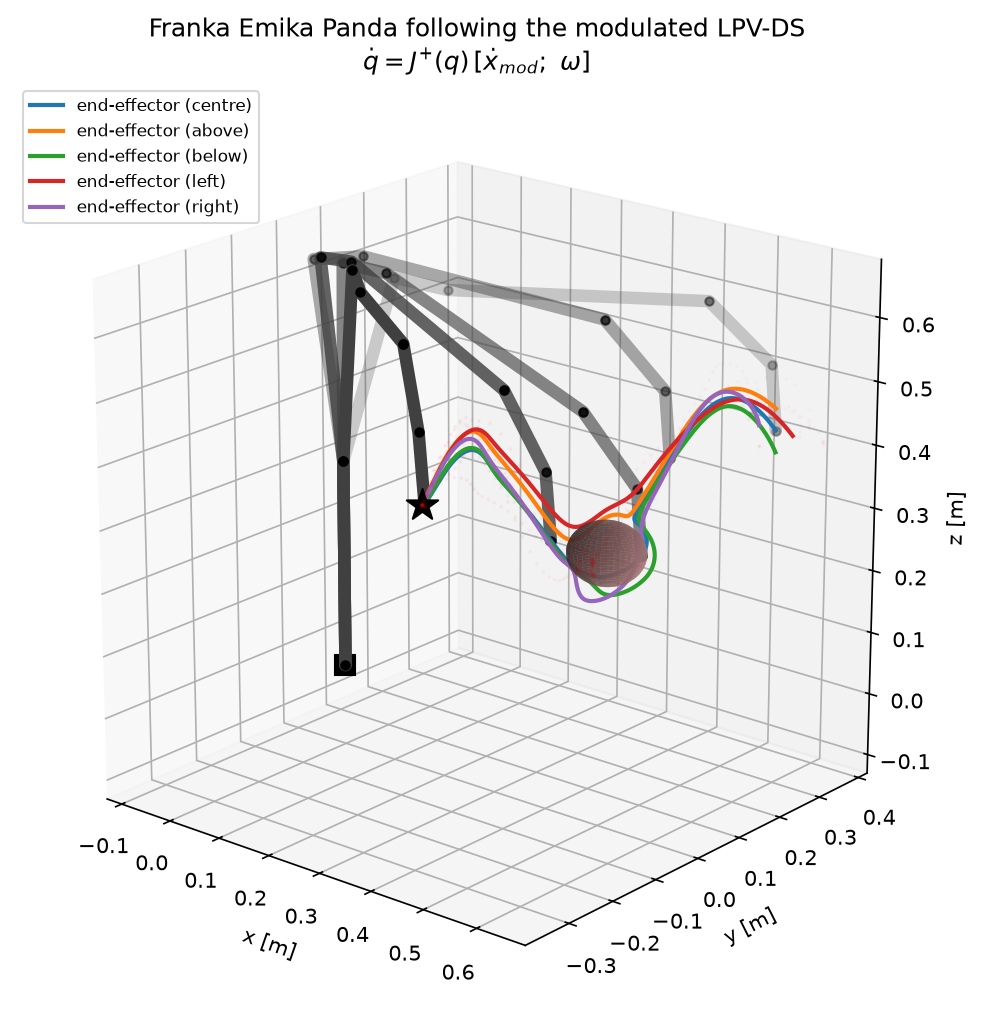
\includegraphics[width=\textwidth]{robot_panda_3d.png}\end{minipage}\hfill
\begin{minipage}{0.64\textwidth}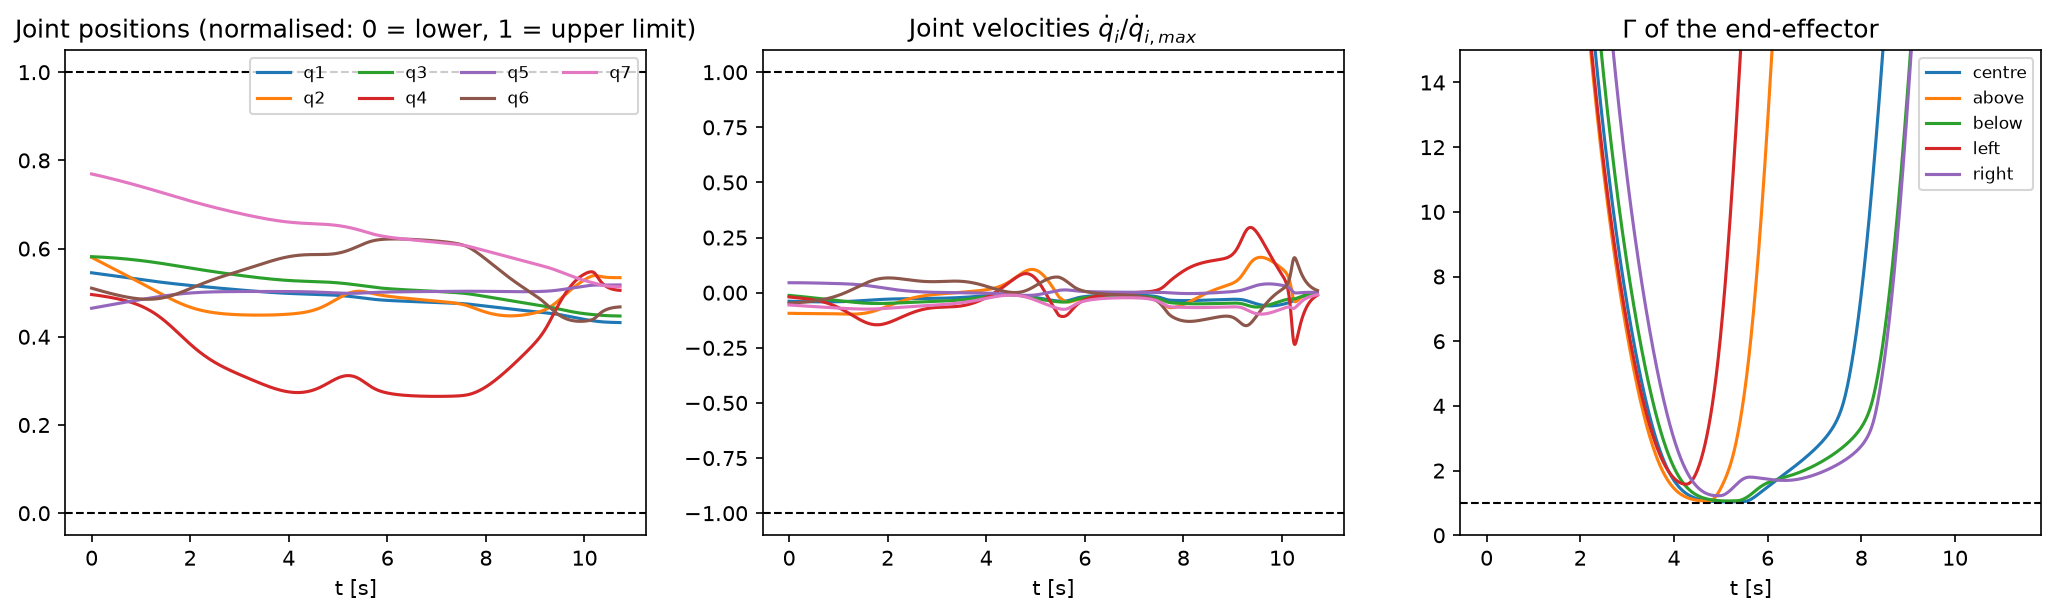
\includegraphics[width=\textwidth]{robot_joints_gamma.png}\end{minipage}
\caption{Franka Panda (Robotics Toolbox) driven by $\dot q=J^{+}(q)[\dot x_{mod};\omega]$. Left: arm
at five instants of the centre run and end-effector paths of all runs. Right: normalised joint
positions and velocities of the centre run (dashed lines are the limits) and $\Gamma$ of the
end-effector for all runs.}
\label{fig:robot}
\end{figure}

% ======================================================= 5. CONCLUSIONS =====
\section{Conclusions}

Combining a learned, provably stable DS with the modulation $M(x)=E D E^{-1}$ gives a controller
that reproduces a demonstrated motion, avoids an obstacle it never saw during training, and still
converges, all without replanning. Two decisions made the biggest difference. The first was learning
$P$ instead of using $P=I$, because a plain QLF could not fit the demonstrated shapes. The second was
clustering the demonstrations by position and direction in 3D.

There are some limitations. Only the end-effector avoids the obstacle, so the wrist or the
links could still touch it (the gripper is vertical and the obstacle is low, so this can happen when
passing under it). The convergence guarantees of the modulation were proven for linear DS, so with a
learned DS a trajectory could in principle stop on the surface. The flow also splits at the point
of the obstacle facing the robot, and starts near that point slide slowly before moving on. Finally,
the robot simulation is kinematic. We did not do the optional extensions (several or moving
obstacles, whole-body avoidance), but the code would allow them: \texttt{modulate} already works for
any star-shaped $\Gamma$.

\paragraph{Use of generative AI.} We used Claude (Anthropic) through Claude Code as a programming
assistant. It helped port the LPV-DS learning from MATLAB to Python, debug the installation, write
the plotting and video scripts, and review the English of this report. We checked the formulation,
the code and every result ourselves.

\small
\begin{thebibliography}{9}\setlength{\itemsep}{0pt}
\bibitem{khansari2011} S. M. Khansari-Zadeh and A. Billard, ``Learning stable nonlinear dynamical systems with Gaussian mixture models,'' \emph{IEEE T-RO}, 27(5), 2011.
\bibitem{khansari2012} S. M. Khansari-Zadeh and A. Billard, ``A dynamical system approach to realtime obstacle avoidance,'' \emph{Autonomous Robots}, 32(4), 2012.
\bibitem{figueroa} N. Figueroa and A. Billard, ``A physically-consistent Bayesian non-parametric mixture model for dynamical system learning,'' CoRL, 2018.
\bibitem{huber2019} L. Huber, A. Billard and J.-J. Slotine, ``Avoidance of convex and concave obstacles with convergence ensured through contraction,'' \emph{IEEE RA-L}, 4(2), 2019.
\bibitem{rtb} P. Corke and J. Haviland, ``Not your grandmother's toolbox: the Robotics Toolbox reinvented for Python,'' ICRA, 2021.
\bibitem{code} Lab code: \texttt{ds-opt}/\texttt{phys-gmm} (N. Figueroa, LASA-EPFL) and \texttt{dynamic\_obstacle\_avoidance} (L. Huber, maintained by A. Prados).
\end{thebibliography}

\end{document}
